\documentclass{article}
\author{}
\usepackage[utf8]{inputenc}
\usepackage{amsmath}
\usepackage{amssymb}
\usepackage{amsmath,amsthm,amssymb,scrextend}
\usepackage{fancyhdr}
\usepackage{graphicx}
\usepackage{hyperref}
\begin{document}

\title{Homework 2 - Dr. Nguyen An Khuong}
\maketitle
\section{Team members}
\begin{itemize}
    \item Ngo Trieu Long
    \item Tang Quoc Thai
    \item Nguyen Trung Thuan
    \item Do Vo Hoang Hung
    \item Nguyen Dinh Khuong
\end{itemize}

\section{Exercises}
\subsection{Exercise 2}
The non-zero singular values are the square roots of the eigenvalues of $A^{T}A$. Whereas, $I^{T}I = I$, and the only eigenvalue of $I$ is 1, therefore, the singular value of $I$ is 1. As we know that compression is done by removing the small singular values, and the singular value of $I$ is 1, therefore, $I$ is not compressible.

One possible rank 5 flag with a 3 by 3 cross of zeros is
\[
    A =
    \begin{bmatrix}
        1 & 0   & 1 & 0   & 0   \\
        0 & 0   & 0 & 1   & 1   \\
        1 & 0   & 1 & 1   & 1   \\
        1 & 1/2 & 1 & 1   & 1   \\
        1 & 1/2 & 1 & 1/2 & 1/2
    \end{bmatrix}
\]


\subsection{Exercise 3}
We can solve this problem using the technique of 'Rank factorization' with the following steps:

\begin{itemize}
    \item Transform the matrix $A$ into its reduced row echelon form $R$ (using Gaussian Elimination).
    \item Choose the pivot columns of $A$ based on the first non-zero entry in each row of $R$.
    \item Choose the non-zero rows of $R$.
\end{itemize}

\[A_{Sweden} =
    \begin{bmatrix}
        1 & 2 & 1 & 1 \\
        2 & 2 & 2 & 2 \\
        1 & 2 & 1 & 1
    \end{bmatrix}
    \equiv
    \begin{bmatrix}
        1 & 0 & 1 & 1 \\
        0 & 1 & 0 & 0 \\
        0 & 0 & 0 & 0
    \end{bmatrix}
\]

The pivot columns are the first and the second columns, and the non-zero rows are the first and the second rows.

\[A_{Sweden} =
    \begin{bmatrix}
        1 & 2 \\
        2 & 2 \\
        1 & 2
    \end{bmatrix}
    *
    \begin{bmatrix}
        1 & 0 & 1 & 1 \\
        0 & 1 & 0 & 0
    \end{bmatrix}
\]

\[A_{Benin} =
    \begin{bmatrix}
        1 & 2 & 2 \\
        1 & 3 & 3
    \end{bmatrix}
    \equiv
    \begin{bmatrix}
        1 & 0 & 0 \\
        0 & 1 & 1
    \end{bmatrix}
\]

The pivot columns are the first and the second columns, and the non-zero rows are the first and the second rows.

\[A_{Benin} =
    \begin{bmatrix}
        1 & 2 \\
        1 & 3
    \end{bmatrix}
    *
    \begin{bmatrix}
        1 & 0 & 0 \\
        0 & 1 & 1
    \end{bmatrix}
\]

\subsection{Exercise 4}
\[
    BB^{T} =
    \begin{bmatrix}
        1 & 2 & 2 \\
        1 & 3 & 3
    \end{bmatrix}
    \begin{bmatrix}
        1 & 1 \\
        2 & 3 \\
        2 & 3
    \end{bmatrix}
    = \begin{bmatrix}
        9  & 13 \\
        13 & 19
    \end{bmatrix}
\]

\[
    Trace(BB^{T}) = 9 + 19 = 28
\]

\[
    Det(BB^{T}) = 9 * 19 - 13 * 13 = 2
\]

\[
    B^{T}B =
    \begin{bmatrix}
        1 & 1 \\
        2 & 3 \\
        2 & 3
    \end{bmatrix}
    \begin{bmatrix}
        1 & 2 & 2 \\
        1 & 3 & 3
    \end{bmatrix}
    = \begin{bmatrix}
        2 & 5  & 5  \\
        5 & 13 & 13 \\
        5 & 13 & 13
    \end{bmatrix}
\]

\[
    Trace(B^{T}B) = 2 + 13 + 13 = 28
\]

\[
    Det(B^{T}B) = 2 * Det(\begin{bmatrix} 13 & 13 \\ 13 & 13 \end{bmatrix}) - 5 * Det(\begin{bmatrix} 5 & 13 \\ 5 & 13 \end{bmatrix}) + 5 * Det(\begin{bmatrix} 5 & 13 \\ 5 & 13 \end{bmatrix}) = 0
\]

With a small singular value $\sigma_{2} \equiv \sqrt{\frac{1}{14}}$, B is compressible.

\subsection{Exercise 5}
\[
    AA^{T}=
    \begin{bmatrix}
        7  & 10 & 7  \\
        10 & 16 & 10 \\
        7  & 10 & 7
    \end{bmatrix}
\]

\[
    Det(AA^{T} - \lambda I) = -\lambda^{3} + 30 \lambda^{2} - 24\lambda
\]

We have $\lambda_{1} = 0$ as the first eigenvalue of $AA^{T}$.

Solving the equation below, we have $\lambda_{2} = 15 + \sqrt{201}$ and $\lambda_{3} = 15 - \sqrt{201}$.

\[
    -\lambda^{2} + 30 \lambda^{} - 24 = 0
\]

So $\sigma_{1} = \sqrt{\lambda_{2}} = \sqrt{15 + \sqrt{201}}$ and $\sigma_{2} = \sqrt{\lambda_{3}} = \sqrt{15 - \sqrt{201}}$.

By using Python we can compute the singular values of $A$ as follows:
\begin{verbatim}
    A = np.matrix([[1, 2, 1, 1], [2, 2, 2, 2], [1, 2, 1, 1]])

    np.set_printoptions(precision=3, suppress=True)
    U, S, V = np.linalg.svd(A)
\end{verbatim}

\[
    A_{Sweden} =
\]
\[
    0.907
    \begin{bmatrix}
        0.517  \\
        -0.682 \\
        0.517
    \end{bmatrix}
    \begin{bmatrix}
        -0.362 & 0.778 & -0.362 & -0.362
    \end{bmatrix}\]
\[
    5.402
    \begin{bmatrix}
        0.482 \\
        0.732 \\
        0.482
    \end{bmatrix}
    \begin{bmatrix}
        0.449 & 0.628 & 0.449 & 0.449
    \end{bmatrix}
\]

\subsection{Exercise 7}
Multiply both sides of $A = U \Sigma V^{T}$ by the matrix $V$ to get $AV = U \Sigma$.

\subsection{Exercise 9}
\begin{verbatim}
    import numpy as np
    import matplotlib.pyplot as plt

    # Generate random matrices
    A = np.random.rand(20, 40)
    B = np.random.randn(20, 40)
    # Compute SVD for A and B
    UA, sigma_A, VA = np.linalg.svd(A, full_matrices=False)
    UB, sigma_B, VB = np.linalg.svd(B, full_matrices=False)

    # Plot singular values with markers
    plt.figure(figsize=(10, 6))
    plt.plot(
        range(1, 21),
        sigma_A,
        marker="o",
        label="Singular Values of A (Uniform Distribution)",
    )
    plt.plot(
        range(1, 21),
        sigma_B,
        marker="s",
        label="Singular Values of B (Normal Distribution)",
    )
    plt.title("Singular Values of Random Matrices A and B")
    plt.xlabel("Singular Value Index")
    plt.ylabel("Singular Value")
    plt.legend()
    plt.grid(True)
    plt.show()
\end{verbatim}

\begin{figure}[ht]
    \centering
    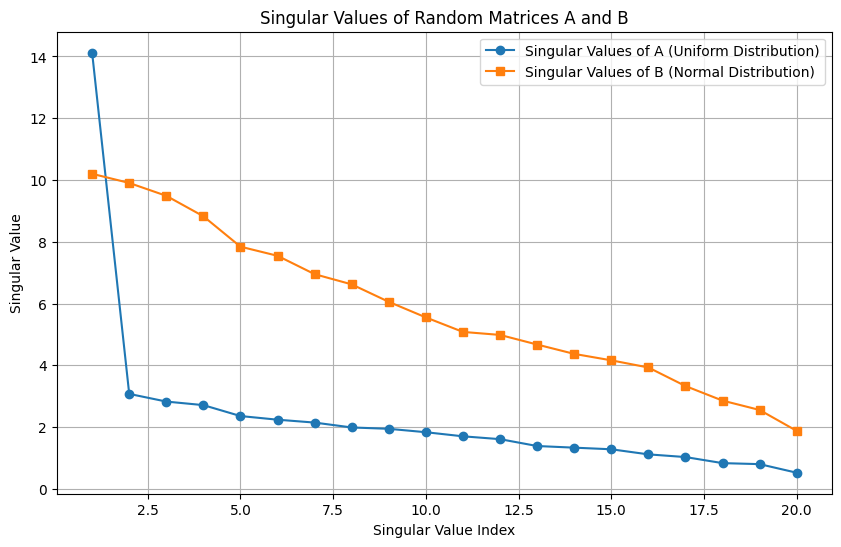
\includegraphics[width=1\textwidth]{img/singular_value_index.png}
    \caption{Comparison of singular values of random matrices A and B}
    \label{fig:singular_value_index}
\end{figure}

The fact that there are 20 singular values for both matrices A and B is because of the following satements:

\begin{itemize}
    \item 20 rows are independent with probability 1, therefore, the rank of both matrices is 20.
    \item A theorem states that the number of singular values of a matrix is equal to the rank of that matrix.
\end{itemize}

Note: the proof of the theorem can be found at \\
\url{https://www.math.ucdavis.edu/~saito/courses/167.f06/svd2.pdf}.

\end{document}
